\documentclass[../thesis.tex]{subfiles}

\begin{document}

\chapter{Predictive Analytics to Support Capacity Planning for Frail and Elderly Patients} \label{chp:predictive}
%\chapter{Classification and Regression Analytics for Frail and Elderly Patients}

\section{Introduction}
Within industry today, OR and predictive analytics are allowing companies to make more informed decisions about their businesses, with the effects of new policies to be understood prior to their implementation. This development has occurred rapidly within healthcare in the 21$^{st}$ century, and with the NHS being one of the UK's and Europe's largest employers, many individuals are now active as healthcare consumers or healthcare providers \cite{NHSJobs2022}. The need for new, more sophisticated technologies and recent demographical changes, such as an ageing population, are the main causes of the rising expenses associated with healthcare treatment \cite{ONS2022}. Patients, as consumers, are no longer prepared to accept subpar services and expect: shorter waiting times, increased appointment availability and faster treatment times \cite{Aiken2021}. By using predictive analytics within healthcare, it allows costs to be minimised and performance to be optimised within the NHS. Predictive analytics uses statistics and modelling techniques to make predictions about future events \cite{Kumar2018}. The analysis of both recent and historical data can help healthcare systems become more dynamic and proactive by looking forward to detect patterns or behaviour.
\begin{description}

\item[\textcolor{red}{Research Aim}] - This chapter will identify predictive techniques which will be applied to the elderly and frail case study within ABUHB, to determine LOS within hospitals. It will seek to create an understanding that will allow the study question, `How do the clinical and demographical attributes of elderly and frail patients affect their duration of stay within hospital?' to be addressed later in this thesis. 
\end{description}

Classification and regression analytics can be applied to the case of frail and elderly patients. To explain how each method operates and is understood, various analytical techniques will be explained in this chapter along with a simplified worked example. Consider a scenario in which the health board receives ten hospital admissions (Table \ref{tab:WEtable}). These patients are elderly (defined as 65 years of age or older) and range in frailty. Seven categories that are typically found in hospital admission data are present in the data. There are two feasible selections for each of the categorical variables. The Royal Gwent Hospital (RGH) and Nevill Hall Hospital (NHH), both of which are found in South East Wales, are the two hospitals that are taken into consideration. Additionally, these patients are admitted to one of two specialities: care of the elderly (COTE) or trauma and orthopaedics (T\&O). Patients may be admitted either as an elective planned admission, or an unplanned emergency admission. The final categorical variable is the admission source, which in this case refers to whether patients are admitted from another hospital or directly from their home. Frailty can be classified into three levels, with level 3 being the most severe case. This is similar to a situation in real life, where the majority of patients have some degree of frailty, while just a few are severely or moderately frail. The patient ages range from 67 to 96, and our final goal is to estimate the length of stay (LOS), which in this case can be one to five days.

\begin{table}[h!]
    \centering
    \begin{adjustbox}{width=\columnwidth}
    \begin{tabular}{cccccccc}\toprule
       \textbf{Patient Number}  & \textbf{Age} & \textbf{Hospital} & \textbf{LOS} & \textbf{Specialty} &\textbf{Admission Method} & \textbf{Admission Source} & \textbf{Frailty Source} \\\midrule
        Patient 1 & 95 & RGH & 5 & COTE & Emergency & Own Home & 3 \\ 
        Patient 2 & 82 & RGH & 3 & COTE & Emergency & Own Home & 2 \\
        Patient 3 & 89 & RGH & 4& T\&O & Emergency & Own Home & 2 \\
        Patient 4 & 87 & RGH & 4 & T\&O & Elective & Own Home & 2 \\
        Patient 5 & 85 & NHH & 3 & COTE & Elective & Transferred & 1 \\
        Patient 6 & 76 & NHH & 1 & COTE & Elective & Transferred & 1\\
        Patient 7 & 71 & NHH & 1 & T\&O & Emergency & Transferred & 1 \\
        Patient 8 & 96 & RGH & 5 & T\&O & Emergency & Own Home & 3 \\
        Patient 9 & 70 & NHH & 1 & COTE & Emergency & Transferred & 1\\
        Patient 10 & 67 & NHH & 1 & T\&O & Elective & Own Home & 1\\\bottomrule
    \end{tabular}
    \end{adjustbox}
    \caption{Worked Example Patient Data - 10 Patients}
    \label{tab:WEtable}
\end{table}

% \[
% \begin{blockarray}{ccccccccc}
%     &\matindex{Age} & \matindex{Hospital} & \matindex{LOS} & \matindex{Specialty} & \matindex{Admission Method}&\matindex{Admission Source} & \matindex{Frailty Level}\\
%     \begin{block}{c(cccccccc)}
%      \matindex{Patient 1}&  95 & RGH & 5& COTE & Emergency & \text{\textit{Own Home}} & 3\\
%      \matindex{Patient 2}&  82 & RGH & 3& COTE& Emergency& \text{\textit{Own Home}} & 2\\
%      \matindex{Patient 3}&  89 & RGH & 4 & T\&O & Emergency& \text{\textit{Own Home}} & 2 \\
%      \matindex{Patient 4}&  87 & RGH & 4 & T\&O& Elective & \text{\textit{Own Home}} & 2\\
%      \matindex{Patient 5}&  85 & NHH & 3 & COTE & Elective& \text{\textit{Transferred}} &1 \\
%      \matindex{Patient 6}&  76 & NHH & 1 & COTE & Elective& \text{\textit{Transferred}} & 1\\
%      \matindex{Patient 7}&  71 & NHH & 1 & T\&O& Emergency& \text{\textit{Transferred}}& 1\\
%      \matindex{Patient 8}&  96 & RGH & 5 & T\&O& Emergency& \text{\textit{Own Home}} & 3\\
%      \matindex{Patient 9}&  70 & NHH & 1 & COTE& Emergency & \text{\textit{Transferred}}&1\\
%      \matindex{Patient 10}&  67 & NHH & 1 & T\&O & Elective & \text{\textit{Own Home}} &1\\
%     \end{block}
%   \end{blockarray}
% \]

Predictive and forecasting techniques were the most frequent study objectives within the healthcare literature, as discussed in Chapter \ref{chp:LiteratureReview}. The studies, however, tended to accomplish this via more traditional OR/MS techniques, such as simulation and Markov chains. The goal of this thesis is to use predictive approaches that are not typically used in healthcare to see if similar patient groups can be found for the frail and elderly.

% This chapter will identify predictive techniques which will be applied to the elderly and frail case study within ABUHB, to determine LOS within hospitals. It will seek to create an understanding that will allow the study question, `How do the clinical and demographical attributes of old and fragile patients affect their duration of stay within hospital?' to be addressed later in this thesis.
The chapter is structured as follows: Section \ref{sec:PredictiveTechniques} will go through the prediction techniques utilised in this thesis, while Section \ref{sec:CART} will discuss classification and regression trees (CART), as well as the extension of random forest metrics. Then, in Section \ref{sec:python} we will determine how these analytical methods can be implemented within Python. A practical example will be demonstrated throughout the chapter to provide a greater understanding of the theory.

% This chapter aims to address the research question 1, `How do the clinical and demographical attributed of elderly and frail patients effect their length of stay within hospital', by using less traditional OR/MS methods. This chapter is structured as follows:


%This thesis examines the use of classification and regression (CART) trees to identify similar groupings of patient attributes.%\hl{TBD - one or two} predictive algorithms. The first method discussed is the application of Classification and regression trees (CART) to group similar attributes together. 


\section{Predictive Techniques}\label{sec:PredictiveTechniques}
Predictive analytics extracts information from existing data using algorithms and machine learning to forecast future events. Predictive analytics can be divided into two subcategories: supervised learning and unsupervised learning.

\subsection{Differences between Supervised and Unsupervised Learning}
To train algorithms for data classification or outcome prediction, supervised learning makes use of labelled datasets. During a `training phase', when data is inputted into the model, patterns within the data are identified and connections between dependent and independent variables are found. In order to demonstrate this relationship, a mathematical equation is created. The training process can produce more accurate outcomes if more data and information is fed into it. Cross-validation then occurs on a `testing' dataset which the model has not been trained upon, to test the accuracy and reliability of the model.

Table \ref{tab:supervised}, contains a collection of the most often used supervised learning methods applied within healthcare, along with relevant healthcare references. 

\begin{table}[h!]
    \centering\scalebox{0.85}{
    \begin{tabular}{ll}\toprule
        \textbf{Method} & \textbf{Healthcare Examples}  \\\midrule
        Regression & Heart Failure Outcomes \cite{Kul}, LOS Prediction \cite{Abe,Welberry} \\
        Classification & Ambulance Delay \cite{Li2022}, Blood Testing \& Donation \cite{Healey2015,SalazarConcha2021} \\
        Naive Bayesian Model & Diabetes Prediction \cite{Shah2021}, Heart Disease Detection \cite{Subbalakshmi2011, Vembandasamy2015}\\
        Random Forest Model & Cancer Prediction \cite{Hanson2019}, Diabetes Detection \cite{Benbelkacem2019,Rallapalli2016}\\
        Neural Networks & Biomedicine \cite{Lakshmanaprabu2019, Lin2016}, Healthcare Access \cite{Chen2022}\\
        Support Vector Machines & Dementia Prediction \cite{Battineni2019}, Stroke Patients \cite{Forkert2015, Kamruzzaman2006}
        \\ \bottomrule
    \end{tabular}}
    \caption{Supervised Learning Methods}
    \label{tab:supervised}
\end{table}

Using supervised learning has various advantages, including improved accuracy levels because the desired result is already known. Supervised approaches are very simple for practitioners without a mathematical background to comprehend and apply in the context of healthcare. However, supervised learning models always require updating in order to keep up with evolving data. The model must repeat the training and validation phases whenever new data variables are added in order to retrain with the new variables. These models can take a long time to compute, especially when employing large amounts of data. If there is unnecessary data included, efficiency may also suffer.

Unsupervised learning, in contrast to supervised learning, does not use labelled data to learn from, instead, the algorithm identifies clusters of similar patterns or groupings. The algorithm will choose the optimal number of classes the data should be divided into because it is unlabelled, therefore it does not need to go through the training and testing stages that supervised learning requires.

The most popular unsupervised learning techniques are shown in Table \ref{tab:unsupervised}, along with real-world healthcare applications. Each technique may incorporate a variety of techniques, for instance, clustering may include, `K-Means', `hierarchical' and `probabilistic' techniques.
\begin{table}[h!]
    \centering\scalebox{0.8}{
    \begin{tabular}{ll}\toprule
        \textbf{Method} & \textbf{Healthcare Examples}  \\\midrule
        Anomaly Detection & Heart Rate Anomalies \cite{Sabic2020,Chauhan2015}, Lung Cancer \cite{Kukita2013}\\
         Clustering & Breast Cancer Recurrence \cite{Belciug2010}, Heart Disease \cite{Shouman2012}, Thyroid Cancer \cite{Liu2011} \\   Dimensionality Reduction& Alzheimer's Diagnosis \cite{Balamurugan2017, Arling}, Diabetic Retinopathy Detection \cite{Gadekallu2020} \\
         \bottomrule
    \end{tabular}}
    \caption{Unsupervised Learning Models}
    \label{tab:unsupervised}
\end{table}

When used in the healthcare industry, unsupervised learning offers a host of advantages, particularly for data that naturally lends itself to labelling. By deciding on the groupings, the unsupervised learning algorithm can save clinicians critical time. Due to the dynamic nature of healthcare data, it is possible to use the algorithms to track how clusters change over time. However because there is no expectation of labelled results, it is uncertain whether the yielded results will be useful. As a result, accuracy levels frequently fall short of those of supervised methods.

Within this research, supervised learning approaches will be examined and applied to the case study of elderly and frail patients. Prescriptive approaches will be used in conjunction with models for regression, classification, and random forests. Discussion into the application of unsupervised methods will take place within Chapter \ref{chp:Discussion}.

\subsection{Generalised Formulation}

\subsubsection{Linear Regression}

Linear regression is used to establish the relationship between a continuous dependent variable and either continuous or discrete independent variables. There are two types of linear regression; simple linear regression in which there is only one independent variable, and multiple linear regression in which there are two or more independent variables.

In a regression problem, the key quantity is the mean value of the outcome, given the value of the independent variable or variables. This quantity is known as the conditional mean, expressed as `$E(Y | x)$' where $Y$ denotes the outcome variable and $x$ denotes a value for the independent variable. In simple linear regression, it is assumed that the conditional mean may be expressed as a linear equation in $x$ as follows \cite{Hosmer1989,Wasserman2004}:
\begin{equation}\label{eq:linreg}
    E(Y | x) = \beta_{0} +\beta_{1}x
\end{equation}
where $\beta_{0}$ is the y-intercept and $\beta_{1}$ is the gradient of the line. 
It is also required for an error term to be including within the equation, denoted $\epsilon$. This error term expresses an observation's deviation from the conditional mean. It is therefore assumed that an observation outcome of the variable may be expressed as \textcolor{blue}{\cite{Hosmer1989, Wasserman2004}}:
\begin{equation}
    y = E(Y | x) + \epsilon
\end{equation}
where $\epsilon$ is the error term.

For multiple linear regression, where multiple independent variables are used to predict the dependent variable, Equation \eqref{eq:linreg} can be modified to include these additional variables \textcolor{blue}{\cite{Hosmer1989}}.
\begin{equation}
    E(Y | x) = \beta_{0} +\beta_{1}x_{1} +\beta_{2}x_{2} + ... +\beta_{n}x_{n}
\end{equation}
Therefore:
\begin{equation}
    y = E(Y | x) + \epsilon
\end{equation}

The findings demonstrate that the dependent variable will increase or decrease by a specific amount for every unit increase in the independent variables. There are four primary assumptions regarding the error value that must be met when using linear regression \textcolor{blue}{\cite{Bowerman2015}}:
\begin{itemize}
    \item The error term values have a mean equal to zero
    \item The error terms have constant variance
    \item The error terms are normally distributed
    \item Each error term is independent from other error terms
\end{itemize}

According to the first three assumptions, the population of potential error term values for each given value of 4x  has a normal distribution with a mean of zero and a variance of $\sigma^{2}$. The final assumption implies that the error terms do not follow a pattern and hence most likely to be independent of one another.

To establish the eligibility for linear regression, the null hypothesis must first be rejected, indicating that there is a relationship to be modelled. For a simple linear regression, the hypotheses are as follows:
\begin{align}
    \text{H}_{0} =& \text{ There is no linear \textcolor{blue}{relationship} (i.e., $\beta_{1} = 0$)}\\
    \text{H}_{1} =&\text{ There is a linear \textcolor{blue}{relationship}  (i.e., $\beta_{1} \neq 0$)}
\end{align}

These hypotheses can be extended for multiple liner regression:
\begin{align}
    \text{H}_{0} =& \text{ There is no linear \textcolor{blue}{relationship} (i.e., all $\beta_{1...n} = 0$)}\\
    \text{H}_{1} =&\text{ There is a linear \textcolor{blue}{relationship} (i.e., at least one $\beta_{1...n} \neq 0$)}
\end{align}
where $n$ is the sample size.

In order to estimate the parameters of the $\beta$ terms, the method of ordinary least squares (OLS) is used. When calculating these terms, OLS first calculates the sum of the squared standard deviations of the observed values of $Y$ before minimising the outcome.

\paragraph{Worked Example}
%\underline{Worked Example}\\
Linear regression can be used to find the relationship connection between a patient's LOS and the dependent variables. Age, with a range of 29 years, is one of the continuous dependent variables. We can ascertain the relationship between LOS and age using a linear regression. The outcomes of the linear regression are shown in Equation \eqref{eq:WElin}. It should be observed that the equation lacks a constant term. The LOS rises by 0.1494 days for every unit increase in age (Figure \ref{fig:WorkedExampleLinReg}). For categorical variable, one-hot encoding is used which results in Equation \eqref{eq:WElog}, if using the variable hospital for prediction. 

\begin{equation}\label{eq:WElin}
    y = 0.1578x -10.1052
\end{equation}
where $x$ is age of the patient. Therefore if the age of a person was 70, their predicted LOS would be 0.9408 days.
\begin{equation}\label{eq:WElog}
    y=1.6667 -0.6667x_{1} +2.3333x_{2}
\end{equation}
where $x_1$ is equal to hospital NHH, and $x_2$ is equal to hospital RGH. Therefore if NHH is attended, then the predicted LOS is 1 day, otherwise RGH is attended and the LOS is 4 days.

\begin{figure}[h!]
    \centering
    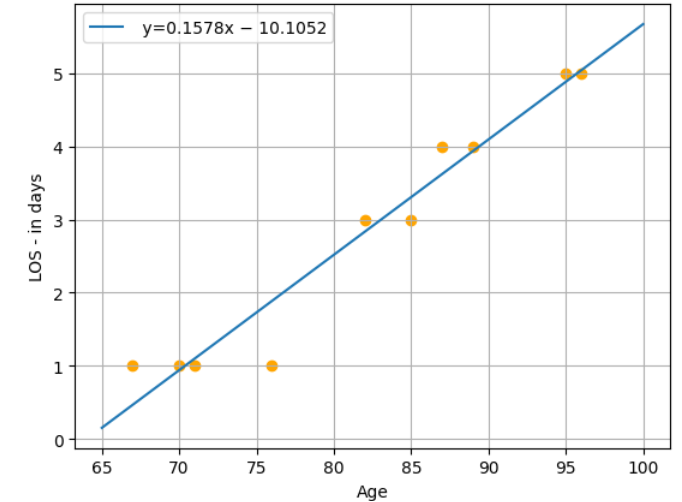
\includegraphics[scale=0.7]{Chapters/Chapter3New/Figures/WorkedExampleLinearReg1.png}
    \caption{Worked Example Linear Regression Equation}
    \label{fig:WorkedExampleLinReg}
\end{figure}


\subsubsection{Logistic Regression}
Dichotomous data is data that has two possible outcomes, data with a binary response in which each participant can only belong to one of the two categories. Applying the conditional mean to dichotomous data requires that it be higher than or equal to zero and less than or equal to one, i.e., $ 0 \leq E(Y|x) \leq 1$. In order to forecast this binary result, logistic regression is applied. The quantity $\textcolor{blue}{\pi(x)} = E(Y|x)$ is used to denote the conditional mean, simplifying the notation. This form of the logistic regression model can be seen within Equation \eqref{eq:logreg} \cite{Hosmer1989,Wasserman2004}.

\begin{equation}\label{eq:logreg}
    \pi(x) = \frac{e^{\beta_{0}+\beta_{1}x}}{1 +e^{\beta_{0}+\beta_{1}x}}
\end{equation}
In order for a linear regression to be fit, a logit transformation of the dependent variable is required to be performed, defined in terms of $\pi(x)$ as follows \cite{Hosmer1989}:
\begin{equation}
    g(x) = \ln \left[ \frac{\pi(x)}{1 - \pi(x)}
    \right]
\end{equation}
\begin{equation}\label{eq:logreg1}
    g(x) = \beta_{0} +\beta_{1}x
\end{equation}
This transformation is important since $g(x)$ is linear in its parameters which may be continuous and range from $-\infty$ to $+\infty$, depending on the range of $x$.
Similar to linear regression, logistic regression also requires an error term for the observation value outcome of the variable, expressed as:
\begin{equation}
    y = \pi(x) + \epsilon
\end{equation}
In order to determine the suitability for logistic regression, the null hypothesis is firstly required to be rejected, suggesting that there is a relationship. The first of these hypotheses is that if $y = 1$ then $\epsilon = 1 - \pi(x)$ with probability $\pi(x)$. Otherwise, $y=0$ and therefore $\epsilon = -\pi(x)$ with probability $ 1- \pi(x)$. Thus, $\epsilon$ has a distribution with mean of zero and variance of equal to $\pi(x)[1-\pi(x)]$. The conditional distribution of the outcome variable follows a binomial distribution with probability given by the conditional mean, $\pi(x)$.

The hypotheses for logistic regression are as follows:
\begin{align}
    \text{H}_{0} =& \text{\textcolor{blue}{All coefficients are zero} (i.e., all $\beta_{1...n} = 0$)}\\
    \text{H}_{1} =& \text{\textcolor{blue}{All coefficients are zero} (i.e., at least one $\beta_{1...n} \neq 0$)}
\end{align}
where n is sample size.

\paragraph{Worked Example}\\
A case study of fifteen patients was used (an additional five rows compared to the previous worked example), to avoid the case of perfect separation and apply this to our worked example. For the remainder of this section, the linear regression will be performed using the initial 10 patient table (Table \ref{tab:WEtable}), while the logistic regression will be performed with the following additional rows added (Table \ref{tab:WETableExtended}).

\begin{table}[h!]
    \centering
    \begin{adjustbox}{width=\columnwidth}
    \begin{tabular}{cccccccc}\toprule
       \textbf{Patient Number}  & \textbf{Age} & \textbf{Hospital} & \textbf{LOS} & \textbf{Specialty} &\textbf{Admission Method} & \textbf{Admission Source} & \textbf{Frailty Source} \\\midrule
        Patient 1 & 95 & RGH & 5 & COTE & Emergency & Own Home & 3 \\ 
        Patient 2 & 82 & RGH & 3 & COTE & Emergency & Own Home & 2 \\
        Patient 3 & 89 & RGH & 4& T\&O & Emergency & Own Home & 2 \\
        Patient 4 & 87 & RGH & 4 & T\&O & Elective & Own Home & 2 \\
        Patient 5 & 85 & NHH & 3 & COTE & Elective & Transferred & 1 \\
        Patient 6 & 76 & NHH & 1 & COTE & Elective & Transferred & 1\\
        Patient 7 & 71 & NHH & 1 & T\&O & Emergency & Transferred & 1 \\
        Patient 8 & 96 & RGH & 5 & T\&O & Emergency & Own Home & 3 \\
        Patient 9 & 70 & NHH & 1 & COTE & Emergency & Transferred & 1\\
        Patient 10 & 67 & NHH & 1 & T\&O & Elective & Own Home & 1\\
        Patient 11 & 89 & RGH & 4 & COTE & Elective & Transferred & 3\\
        Patient 12 & 70 & NHH & 1 & COTE & Elective & Own Home & 2\\
        Patient 13 & 75 & NHH & 4 & T\&O & Elective & Transferred & 3\\
        Patient 14 & 72 & NHH & 2 & COTE & Elective & Transferred & 3\\
        Patient 15 & 87 & RGH & 5 & COTE & Emergency & Own Home & 2\\\bottomrule
    \end{tabular}
    \end{adjustbox}
    \caption{Worked Example Patient Data - 15 Patients}
    \label{tab:WETableExtended}
\end{table}

Given that logistic regression requires a grouped variable to predict outcomes, LOS can be divided into groups of `$<$ 4 days' and `$\geq$ 4 days, to identify the groupings of patients which have longer LOS's in hospital.

Performing the logistic regression with age as a continuous variable, Equation \eqref{eq:logreg1} is generated.
\begin{equation}\label{eq:logreg1}
y = 0.2661x-21.7946
\end{equation}
Therefore, for a patient who was aged younger than 82, they would fall into category `0' and their LOS would be predicted to be less than 4 days. Otherwise, for those aged 82 and over, they would be predicted to fall into the category of `1' and have a LOS equal to or greater than 4 days.

Performing with hospital as a categorical variable, results in the following:
\begin{equation}\label{eq:logreg2}
y = 2.8904x_{RGH} -1.7918 
\end{equation}
Within this calculation, the intercept did not have a significant p-value (0.097), and therefore can be considered as zero.

This means, for patients who attend NHH hospital, the predicted grouping would be `0' and therefore have a LOS of less than 4 days. RGH patients would result in $y \geq 1$ and would therefore fall into group `1'.


\subsection{Evaluation Metrics}
In order to determine the success of using model against the data, traditional scoring techniques will be used for both the linear and logistic regressions.

For linear regression, two scoring measures will be used for evaluation of the models:

\begin{enumerate}
    \item R$^{2}$ Value
    \item Adjusted R$^{2}$ Value
\end{enumerate}

The theory behind these two scoring methods are discussed below.

\subsubsection{R$^{2}$ Value}\\
 The R$^{2}$ is the coefficient of determination and calculates how good a model's fit is compared to a given dataset. It indicates how close the predicted values are to the actual values.

\begin{equation}\label{eq:r2value}
    \text{R}^{2} =  1 - \frac{SS_{RES}}{SS_{TOT}} = 1 - \frac{\sum_{i}(y_{i} - \hat y_{i})^{2}}{\sum_{i}(y_{i} - \bar y)^{2}}
\end{equation}

where $SS_{RES}$ is the sum of square of the residuals and $SS_{TOT}$ is the total sum of squares. Further expanding into the formula for $SS_{RES}$, $y_{i}$ is the observed variable value and $\hat y_{i}$ is the value estimated by the regression line. Similarly for $SS_{TOT}$, $y_{i}$ is the observed variable value and $\bar y$ is the mean value.
The range for the R$^{2}$ value is between -$\infty$ to 1, where a negative value indicated the best fit line is performing worse than the average fit line.

\paragraph{Worked Example}\\
When calculating the $R^{2}$ value for the linear regressions performed in the worked example, we can use Equation \eqref{eq:WElin}.
Starting with patient 1 who is aged 95, their recorded LOS was 5 with a predicted LOS of 4.8858 days. $SS_{RES}$ can be calculated as follows:

\begin{align}
    \hat y =& -10.1052 + 0.1578x \tag{\ref{eq:WElin} revisited}\\
    \hat y =& -10.1052 + (0.1578* 95) \approx 4.8858 \\
    (y_{i} -\hat y_{i})^{2} =& (5-4.8858)^{2} = 0.0013
   % (y_{i} -\hat y_{i})^{2} =& 0.0013
\end{align}
This process is performed for all ten patients, resulting in an $SS_{RES}$ value of 1.3674.
\begin{equation}
    \sum (y_{i} - \hat y_{i})^2 = 1.3674
\end{equation}
Then we can calculate the $SS_{TOT}$, by using the equation $ \bar y = \frac{\sum y}{n}$. Since there are 10 samples within the data, and the total LOS sums to 29, our $\bar y$ value is 2.9. 
\begin{align}
    (y_{i} -\bar y)^{2} =& (5-2.9)^2 = 4.41
\end{align}
Similarly this process continues for all ten patients:
\begin{equation}
    \sum(y_{i} -\bar y)^{2} = 25.7
\end{equation}
Therefore using Equation \eqref{eq:r2value}, we can calculate the $R^2$ value to be:
\begin{align}
    R^{2} &= 1 - \frac{1.3674}{25.7} = 0.9468
\end{align}
Therefore the age accounts of 94.68\% of the variation in the LOS.

Categorical variables follow a similar process using Equation \eqref{eq:WElog}

\begin{equation}
    \hat y=1.6667 -0.6667x_{1} +2.3333x_{2}\tag{\ref{eq:WElog} revisited}
\end{equation}

For each patient, either $x_{1}$ or $x_{2}$ will be given a value of 1, with the other being zero to calculate $\hat y$.
\begin{align}
    \hat y &= 1.6667 -0.6667(0) +2.3333(1) = 4\\
    (y_{i} - \hat y_{i})^2 &= (5-4)^2 
\end{align}
To compute $SS_{RES}$, this procedure can be repeated for all ten cases.
\begin{equation}
    \sum(y_{i} - \hat y_{i})^2 = 4
\end{equation}
Since the value of the $SS_{TOT}$ remains unchanged from the previous calculation, $R^{2}$ is determined as follows:
\begin{align}
    R^{2} &= 1 - \frac{4}{25.7}  = 0.8444
\end{align}


\subsubsection{Adjusted R$^{2}$ Value}\\
The adjusted R$^{2}$ value is a modification of R$^{2}$ value that accounts for variables that are not significant in the model. The adjusted R$^{2}$ determines the extent of the variance of the dependent variable which is explained by the independent variable.

\begin{equation}\label{eq:adjr2}
    \text{R}^{2}_{adj} = 1 - \left[ \frac{(1-\text{R}^{2})(n-1)}{n-k-1}\right]
\end{equation}
where $n$ is the number of points in the sample and $k$ is the number of independent variables in the model.

\paragraph{Worked Example}\\
The calculated $R^{2}$ for the worked example was 0.9468. This value can be entered into the Equation \eqref{eq:adjr2}, to calculate the adjusted $R^{2}$ value.

\begin{equation}
    \text{R}^{2}_{adj} &= 1 - \left[ \frac{(1-0.9468)(10-1)}{10-1-1}\right] = 0.9401 \\
\end{equation}



Therefore the adjusted $R^{2}$ value is 94.01\%.

Similarly, the adjusted $R^{2}$ value for the hospital attended can be determined using the following formula:

\begin{equation}
    R^{2}_{adj}  &= 1 - \left[ \frac{(1-0.8444)(10-1)}{10-1-1}\right] = 0.8249    
\end{equation}
%https://www.ritchieng.com/machine-learning-evaluate-linear-regression-model/

To evaluate how well the model fits the data in logistic regression, error measures are also required. The following are the four primary evaluation metrics in logistic regression that are used to determine accuracy and error rates and are as follows:
\begin{enumerate}
    \item Confusion Matrix
    \item Classification Report
    \item Accuracy Score
    \item Receiver Operating Characteristic Curve (ROC curve)
\end{enumerate}

The data utilised in this thesis will be subjected to these four measurement methodologies.

\subsubsection{Confusion Matrix}\\
The number of values that are successfully or incorrectly predicted is determined from the confusion matrix. It is possible to distinguish between type I and type II errors using Table \ref{tab:ConfusionMatrix}.
% \begin{table}[h!]
% \centering
% \begin{tabular}{cccc}\cline{1-4}
% \multicolumn{1}{|c|}{\multirow{4}{*}{\textbf{\textcolor{blue}{Predicted}}}} & \multicolumn{3}{c|}{\textbf{\textcolor{blue}{Actual}}}\\ \cline{2-4}
% \multicolumn{1}{|c|}{}& \multicolumn{1}{c|}{}         & \multicolumn{1}{c|}{\textcolor{red}{Positive}} & \multicolumn{1}{c|}{\textcolor{red}{Negative}}       \\ \cline{2-4}
% \multicolumn{1}{|c|}{}& \multicolumn{1}{c|}{\textcolor{red}{Positive}} & \multicolumn{1}{c|}{True Positive (TP)}&\multicolumn{1}{l|}{False Positive (FP)}              \\ \cline{2-4}
% \multicolumn{1}{|c|}{}&\multicolumn{1}{c|}{\textcolor{red}{Negative}} & \multicolumn{1}{l|}{False Negative (FN)}         & \multicolumn{1}{c|}{True Negative (TN)}              \\      \cline{1-4}        
% \end{tabular}
% \caption{Confusion Matrix}
% \label{tab:ConfusionMatrix}
% \end{table}

\begin{table}[]
    \centering
    \begin{tabular}{clccc} \toprule
    && \multicolumn{2}{c}{\textbf{Predicted Value} }\\
         && \textbf{Positive} & \textbf{Negative}  \\ \midrule
      \multirow{2}{*}{\textbf{Actual Value}} &\textbf{Positive}   & True Positive (TP) & False Negative (FN)   \\
      &\textbf{Negative}  & False Positive (FP) & True Negative (TN)\\ \bottomrule
    \end{tabular}
\caption{Example Confusion Matrix}
\label{tab:ConfusionMatrix}
\end{table}
% \begin{table}[h!]
% \centering
% \begin{tabular}{c >{\bfseries}r @{\hspace{0.8em}}c @{\hspace{0.4em}}c @{\hspace{0.8em}}l}
%   \multirow{10}{*}{\rotatebox{90}{\parbox{1.1cm}{\bfseries\centering Actual\\ Value}}} & 
%     & \multicolumn{2}{c}{\bfseries Prediction Outcome} & \\
%   & & \bfseries p & \bfseries n & \bfseries total \\
%   & p$'$ & \MyBox{True}{Positive (TP)} & \MyBox{False}{Negative (FN)} & P$'$ \\[2.4em]
%   & n$'$ & \MyBox{False}{Positive (FP)} & \MyBox{True}{Negative (TN)} & N$'$ \\
%   & total & P & N &
% \end{tabular}
% \caption{\textcolor{blue}{Example Confusion Matrix}}
% \label{tab:ConfusionMatrix}
% \end{table}

False positives (FP), also known as type I errors, occur when a result that should be negative turns out to be positive. As patients who are not diagnosed may be discharged from the care pathway, these errors are frequently considered worse in the application of healthcare. As a result, individuals can be denied access to treatment. False negatives (FN), or type II  errors, occur when a result is projected to be positive however really turns out to be negative. Patients may experience anxiety due to misdiagnosis, but this would be detected and fixed further along the care pathway.

\paragraph{Worked Example}

With fifteen patients, we may analyse the aggregated LOS against age using logistic regression. The findings are displayed in Table \ref{tab:ConfusionMatrixEX1} and demonstrate that the model correctly predicts the majority of situations since there is only one type I error and two type II errors.

An identical confusion matrix is produced when the logistic regression is performed for the categorical variable hospital, (Table \ref{tab:ConfusionMatrixEX1}), allowing the same conclusions to be drawn.

\begin{table}[]
    \centering
    \begin{tabular}{clccc} \toprule
    && \multicolumn{2}{c}{\textbf{Predicted Value} }\\
         && \textbf{Positive} & \textbf{Negative}  \\ \midrule
      \multirow{2}{*}{\textbf{Actual Value}} &\textbf{Positive}   & 6 & 2   \\
      &\textbf{Negative}  & 1 & 6\\ \bottomrule
    \end{tabular}
\caption{\textcolor{blue}{Confusion Matrix for Worked Example}}
\label{tab:ConfusionMatrixEX1}
\end{table}

% \begin{table}[h!]
% \centering
% \begin{tabular}{cccc}\cline{1-4}
% \multicolumn{1}{|c|}{\multirow{4}{*}{\textbf{\textcolor{blue}{Actual}}}} & \multicolumn{3}{c|}{\textbf{\textcolor{blue}{Predicted}}}\\ \cline{2-4}
% \multicolumn{1}{|c|}{}& \multicolumn{1}{c|}{}         & \multicolumn{1}{c|}{\textcolor{red}{Positive}} & \multicolumn{1}{c|}{\textcolor{red}{Negative}}       \\ \cline{2-4}
% \multicolumn{1}{|c|}{}& \multicolumn{1}{c|}{\textcolor{red}{Positive}} & \multicolumn{1}{c|}{6}&\multicolumn{1}{c|}{2}              \\ \cline{2-4}
% \multicolumn{1}{|c|}{}&\multicolumn{1}{c|}{\textcolor{red}{Negative}} & \multicolumn{1}{c|}{1}         & \multicolumn{1}{c|}{6}              \\      \cline{1-4}        
% \end{tabular}
% \caption{Confusion Matrix}
% \label{tab:ConfusionMatrixEX1}
% \end{table}


\subsubsection{2. Classification Report}\\
The second set of metrics focuses on three parameters, which are derived using Table \ref{tab:ConfusionMatrix}. These are the precision, recall and f1 scores \cite{Baratloo2015}.
\begin{equation}\label{eq:precision}
    \text{Precision} = \frac{TP}{TP + FP}
\end{equation}
\begin{equation}\label{eq:recall}
    \text{Recall} = \frac{TP}{TP + FN}
\end{equation}

\begin{equation}
 \text{F1 Score} = 2 * \frac{(\frac{TP}{TP + FP}) *(\frac{TP}{TP + FN})}{(\frac{TP}{TP + FP}) + (\frac{TP}{TP + FN})}
\end{equation}
Or equivalently:
\begin{equation}\label{eq:f1score}
    \text{F1 Score} = 2 * \frac{Precision * Recall}{Precision + Recall}
\end{equation}
The precision is defined by the number positive results correctly predicted by the total number within the predicted positive class. The recall score is calculated by dividing the total number of correctly predicted positive results by the number of real positive results. The F1 Score, is defined as the harmonic mean between the precision and recall values.

\paragraph{Worked Example}\\
The following precision, recall and F1 score will be the same because the confusion matrix produced by the linear and logistic regressions (Table \ref{tab:ConfusionMatrixEX1}) was the same.

We may infer the following values from the confusion matrix: TP = 6, FP = 2, FN = 1 and TN =6. Consequently, the following are the precision, recall and F1 scores:

\begin{align}
    \text{Precision} &= \frac{6}{6+2}= 0.75\\
    \text{Recall} &= \frac{6}{6+1}= 0.8571\\
    \text{F1 Score} &= 2 * \frac{\frac{6}{8} * \frac{6}{7}}{\frac{6}{8} + \frac{6}{7}}= 0.8
\end{align}

All three results are greater than 70\%, demonstrating the model's ability to correctly forecast the LOS categories.

\subsubsection{Accuracy Score}\\
The proportion of correctly classified predictions over all of the predictions is known as the accuracy. Equation \eqref{eq:accuracy} can be used to express this \cite{Baratloo2015}.

\begin{equation}\label{eq:accuracy}
    \text{Accuracy} = \frac{TN + TP}{TN + FP + TP + FN}
\end{equation}

A balanced distribution of the data is important when considering accuracy as a scoring criterion. When there is an imbalance in the dataset, the prediction frequently skews the findings significantly so that they fall into one of the predicted categories. A high accuracy result would be the outcome from this.

\paragraph{Worked Example}\\
The accuracy can be determined once more by using the confusion matrix from the previous calculation.

\begin{align}
    \text{Accuracy}  &= \frac{6+6}{6+2+1+6}= 0.8
\end{align}

An accuracy score of 80\% shows that patients are appropriately assigned to the LOS group that 80\%.


\subsubsection{ROC Curve}\\
The ROC curve, which displays the TP rate against the FP rate at various classification thresholds, is the final metric. An example ROC curve and its related area under the curve (AUC) value are shown in Figure \ref{fig:Example-ROCCurve}. The model receives a score between 0 and 1, with the higher the AUC value, the greater the percentage of properly predicted values.

\begin{figure}[h!]
    \centering
    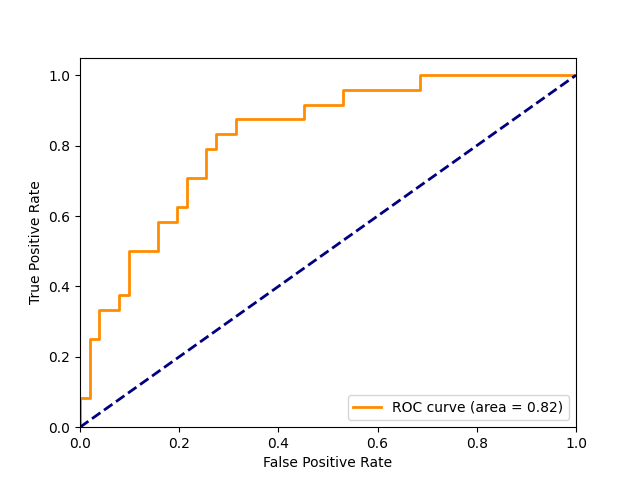
\includegraphics[scale=0.65]{Chapters/Chapter3New/Figures/ROC Curve Example.png}
    \caption{Example ROC Curve}
    \label{fig:Example-ROCCurve}
\end{figure}

\paragraph{Worked Example}\\
In Figures \ref{fig:ROC1} and \ref{fig:ROC2}, the ROC curves are displayed. The AUC for the age example was 80.36\%, which indicates that a large percentage of projected values are successfully predicted. The higher AUC value of 94.64\% implies that the hospital variable is more effective at predicting the LOS group when directly compared to the age example.


\begin{figure}
\centering
\begin{minipage}{.5\textwidth}
  \centering
  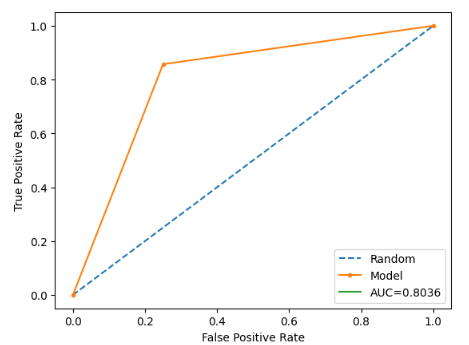
\includegraphics[height = 5cm]{Chapters/Chapter3New/Figures/ROCCurveExample.png}
  \captionof{figure}{ROC Curve for\\ Continuous Age and LOS Prediction}
  \label{fig:ROC1}
\end{minipage}%
\begin{minipage}{.5\textwidth}
  \centering
  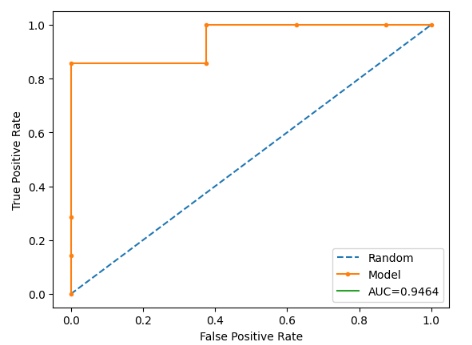
\includegraphics[height = 5cm]{Chapters/Chapter3New/Figures/ROCCurveExample1.png}
  \captionof{figure}{ROC Curve for Categorical Hospital and LOS Prediction}
  \label{fig:ROC2}
\end{minipage}
\end{figure}


This subsection has described the scoring criteria for both linear and logistic regressions and shown how these models function with worked examples of ten and fifteen patients, respectively. Chapter \ref{chp:Experimental Analysis} of this thesis will further apply these predictive analytics to a dataset of elderly and frail patients.


\section{Classification and Regression Trees}\label{sec:CART}
Classification and regression trees (CART) are a data mining technique in which variables predict an outcome. The parameters that make up the final groups are visually represented by a decision tree. The decision tree asks a series of questions that decide the groups into which the data is sorted. CART models are a form of binary recursive partitioning, where each node is split into two groups.

In data mining, a decision tree is a prediction model that may be applied to both classifiers and regression models in data mining. In contrast, the term `decision tree' in operations research refers to the hierarchical model of decisions and their consequences.

CART is comprised of four main components. The dependent variable that the algorithm seeks to predict is the first element. The second component are the independent variables that are related to, and used to predict the dependent variable. The third component is the training dataset, a subset of the main dataset that includes both the dependent and independent variables. This is used to train and allow the algorithm to learn. The testing dataset, which is the final component, will assess the precision and reliability of the algorithm's predictions.

The decision tree illustrates the clinical judgements required to reach the final classification grouping. It is composed of root, decision and terminal nodes. The tree's root node, which symbolises the whole population, is at the top of the structure. The population is then divided up into decision or terminal nodes based on certain criteria. The tree's terminal nodes, which hold the information indicating to which grouping the data belongs, are located at its very end.

Depending on the maximum tree depth or the maximum number of leaves (terminal nodes) in the model, the tree's size will vary. Figure \ref{Fig:ExampleDT1} displays a decision tree with a max depth of one or two maximum leaves.

\begin{figure}[h!]
\centering
\begin{tikzpicture}[scale=0.75, transform shape,node distance=4.2cm]

\node (start1)[startstop]  {\parbox{3cm}{\centering Root Node} };

\node (pro1)[term, below left of = start1]{\parbox{3cm}{\centering Terminal Node}} ;
\node (pro2)[term, below right of = start1]{\parbox{3cm}{\centering Terminal Node}};
\draw [arrow] (start1) -- node [anchor=east]{\begin{tabular}{c} Yes \end{tabular}}
 (pro1);
\draw[arrow] (start1) -- node [anchor=west]{\begin{tabular}{c} No \end{tabular}}(pro2);

\end{tikzpicture}
    \caption{Example Decision Tree Split}
    \label{Fig:ExampleDT1}
\end{figure}

The depth or maximum number of leaves can be increased to guarantee that there are more splits (see Figure \ref{Fig:ExampleDT2}). From this, the following rules can be deduced:

\begin{enumerate}
    \item If (Root-Node = True) AND (Decision-Node-1 = True) THEN Terminal-Node-1 = True
    \item If (Root-Node = True) AND (Decision-Node-1 = False) THEN Terminal-Node-2 = True
    \item If (Root-Node = False) AND (Decision-Node-2 = True) THEN Terminal-Node-3 = True    
    \item If (Root-Node = False) AND (Decision-Node-2 = False) AND (Decision-Node-3 = True) Then Terminal-Node-4 = True
    \item If (Root-Node = False) AND (Decision-Node-2 = False) AND (Decision-Node-3 = False) Then Terminal-Node-5 = True   
\end{enumerate}



\begin{figure}[h!]
\centering
\begin{tikzpicture}[scale=0.75, transform shape,node distance=4.2cm]

\node (start1)[startstop]  {\parbox{3cm}{\centering Root Node} };

\node (pro1)[process, below left of = start1]{\parbox{3cm}{\centering Decision Node 1}} ;

\node (pro3)[term, below left of =  pro1]at (-2,-2) {\parbox{3cm}{\centering Terminal Node 1}};

\node (pro4)[term, below right of =  pro1]at(-4.5,-2) {\parbox{3cm}{\centering Terminal Node 2}};

\node (pro2)[process, below right of = start1]{\parbox{3cm}{\centering Decision Node 2}};

\node (pro6)[term, below left of =  pro2]at (5,-2)  {\parbox{3cm}{\centering Terminal Node 3}};


\node (pro7)[process,below right of = pro2]at (2.5,-2)  {\parbox{3cm}{\centering Decision Node 3} };

\node (pro8)[term,below right of = pro7]at (4.5,-4)  {\parbox{3cm}{\centering Terminal Node 5} };

\node (pro9)[term,below right of = pro7]at (1,-4)  {\parbox{3cm}{\centering Terminal Node 4} };

\draw [arrow] (start1) -- node [anchor=east]{\begin{tabular}{c} Yes \end{tabular}}
 (pro1);
\draw[arrow] (start1) -- node [anchor=west]{\begin{tabular}{c} No \end{tabular}}(pro2);
\draw[arrow] (pro1) -- node [anchor=west]{\begin{tabular}{c} Yes \end{tabular}}(pro3);
\draw[arrow] (pro1) -- node [anchor=west]{\begin{tabular}{c} No \end{tabular}}(pro4);
\draw[arrow] (pro2) -- node [anchor=west]{\begin{tabular}{c} Yes \end{tabular}}(pro6);
\draw[arrow] (pro2) -- node [anchor=west]{\begin{tabular}{c} No \end{tabular}}(pro7);
\draw[arrow] (pro7) -- node [anchor=west]{\begin{tabular}{c} No \end{tabular}}(pro8);
\draw[arrow] (pro7) -- node [anchor=west]{\begin{tabular}{c} Yes \end{tabular}}(pro9);
\end{tikzpicture}
    \caption{Extension of Example Decision Tree Split}
    \label{Fig:ExampleDT2}
\end{figure}

The algorithm determines the most important splitting criteria in order to gain the most information.


\subsection{Generalised Formulation}
Within both regression and classification trees, categorical variables are present within the data. Because of the nature of the algorithm, the variables have to undergo preprocessing to change these to numerical data. Since there is no ordinal relationship in the categorical data, one-hot encoding must be used instead of integer encoding. Each distinct integer value is represented by a brand-new binary variable, which replaces the categorical variable.

The newly one-hot encoded variables can the be run with the numerical variables into the CART algorithm. 

\subsubsection{Regression Trees}
A continuous outcome variable is predicted via regression trees. The regression algorithm known as \textit{`DecisionTreeRegressor'} is part of the machine learning toolkit called `Scikit-Learn' \cite{Pedregosa2011} in Python. Regression trees can be created and developed as a result.

The decision-making process of the algorithm is based on the mean square error (MSE), which also helps to establish the final groupings of data. The MSE informs the user as to how much their prediction deviates from the original target (Equation \eqref{Eq:MSE1}) \cite{Karunasingha2022}. Since regression trees are aiming to predict a continuous variable, once the final groupings are determined, the average of the dependent variable is calculated.

\begin{equation}\label{Eq:MSE1}
    \text{MSE} = \frac{1}{n}\sum^{n}_{i=1}(Y_{i} - \hat{Y}_{i})^2
\end{equation}
where $Y$ is the actual value and $\hat{Y}$ is the prediction.
The $R^{2}$ value determines the coefficient of determination of the prediction, given in Equation \eqref{Eq:R2}.

The process of creating a regression tree is described by Algorithm \ref{Alg:Regression}.

\begin{algorithm}
\caption{Regression Tree}\label{Alg:Regression}
Determine stopping criterion:\\ $max\_depth, min\_samples\_split, min\_samples\_leaf, min\_weight\_fraction\_leaf,$\\$ max\_leaf\_nodes, min\_impurity\_decrease$\\
Start with a single node n containing all points. \\
Calculate $MSE^{n}$\\
\While{MSE^{n}>0 \normalfont{\textbf{ or}} \textit{ stopping criterion not met}}{
k = \text{number of binary splits}\\
\For{a = 1 to k}{
Calculate MSE^{n}_{a} \\
x_{a} = MSE^{n} - MSE^{n}_{a}\\
}
\text{Set MSE^{n} = \textit{Max(} $x_{a}$)
}\\
\textit{Create two new nodes, n' and n'' and calculate new Gini-Index for each}}
\end{algorithm}

% \begin{algorithm}
% \caption{Regression Tree}\label{Alg:Regression}
% 1. {Start with a single node containing all points}. \\
% \hspace{1cm} Calculate the MSE. \\

% 2. If all points in the node have the same value for all the input variables,\\ \hspace{0.3cm} STOP.\\
% \hspace{0.3cm} Otherwise, search over all binary splits of all variables for the one which will \\
% \hspace{0.3cm} reduce MSE as much as possible. If the largest decrease in MSE would be \\
% \hspace{0.3cm} less than some threshold $\delta$, or one of the resulting nodes would contain less \\
% \hspace{0.3cm} than $q$ points, STOP. \\
% \hspace{0.3cm} Otherwise, take that split, creating two new nodes.\\
% 3. In each new node, go back to step 1.
% \end{algorithm}

A decision tree of the regression algorithm can then be constructed to provide the user with a visual representation of the clinical decisions.

\paragraph{Worked Example}\\
Reverting to the prior example, we apply Algorithm \ref{Alg:Regression} to forecast the continuous LOS for the fifteen hospitalised patients. 

Figure \ref{fig:RegTree1} shows a regression tree with a test set size of 20\% and a maximum of four leaf nodes. For the leaf nodes where the MSE is equal to zero, $Y_{i} - \hat Y_{i}$ is also equal to zero and therefore there is a perfect prediction. The figure also shows that the most crucial element in deciding a patient's LOS is whether they are 86 years old or younger. The LOS is represented by colours, and the shorter the LOS, the lighter the colour. The colours associated depict the LOS, and the lighter the colour indicates the shorter the LOS. The node with the value 4.5, is the one with the darkest colour, indicating that this has the longest LOS prediction in the model.

\begin{figure}
    \centering
    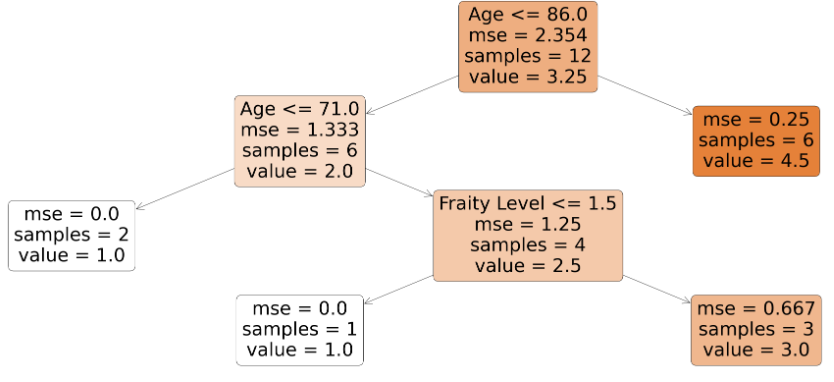
\includegraphics[scale = 0.8]{Chapters/Chapter3New/Figures/RegTree1.png}
    \caption{Regression Tree for Worked Example}
    \label{fig:RegTree1}
\end{figure}

%Due to the nature of only having a small number of patients and a small range of LOS, the predictive ability is very good, and in this example predicts the LOS perfectly.

\subsubsection{Classification Trees}
When the dependent variable is categorical and the tree algorithm seeks to predict the class, classification trees are utilised. The classification technique, \textit{`DecisionTreeClassifier'}, can be used with the Scikit-Learn \cite{Pedregosa2011} Python library. Although classification trees adopt a methodology very similar to that of regression trees, MSE should not be applied because they forecast a categorical outcome variable. Instead, the optimum splitting choice is determined using the Gini Index or Gini impurity. The Gini Index yields a number between 0 and 1, with a smaller value indicating greater sample homogeneity. The Gini Index is calculated using Equation \eqref{eq:Gini}, which involved subtracting the sum of the squared probabilities of each class from one \cite{Das2020}.

\begin{equation}\label{eq:Gini}
    \text{Gini Index} = 1 - \sum_{i=1}^{n}p_{i}^{2}
\end{equation}
where $i$ is the number of classes and $p_{i}$ is the probability of an object that is being classified to a particular class.

Algorithm \ref{Alg:Classification} illustrates the steps involved in creating a classification tree and has been extended from Algorithm \ref{Alg:Regression}.
\begin{algorithm}
\caption{Classification Tree}\label{Alg:Classification}
Determine stopping criterion:\\ $max\_depth, min\_samples\_split, min\_samples\_leaf, min\_weight\_fraction\_leaf,$\\$ max\_leaf\_nodes, min\_impurity\_decrease$\\
Start with a single node n containing all points. \\
Calculate Gini-Index$^{n}$\\
\While{{Gini-Index$^{n} >$}0  \normalfont{\textbf{or}}\textit{ stopping criterion not met}}{
k = \text{number of binary splits}\\
\For{a = 1 to k}{
Calculate Gini-Index$^{n} _{a}$ \\
x_{a} = \text{Gini-Index}$^{n}$ - \text{Gini-Index}$^{n} _{a}$\\
}
\text{Set Gini-Index}$^{n}$ = \textit{Max} ($x_{a}$)
\\
\textit{Create two new nodes, n' and n'' and
calculate new Gini-Index for each}}
\end{algorithm}

\paragraph{Worked Example}
For the classification tree, patients were split into two groups based on their LOS: those admitted for 4 days or less and those admitted for 4 days or more. Once more, a test set of 20\% was used.

The classification tree is depicted in Figure \ref{fig:classificationtreeExample}, where the maximum number of leaf nodes is set to four. Using the training data, perfect prediction occurs since all four end nodes have a Gini Index of zero. The regression tree's findings (Figure \ref{fig:RegTree1}) showed that a patient's age was the primary determinant in identifying the LOS group. The rest of the tree breaks differently, though. The number of patients that fit into a certain node is indicated by the colour depth in the diagram. White nodes show an equal distribution of patients inside that node.

\begin{figure}[h!]
    \centering
    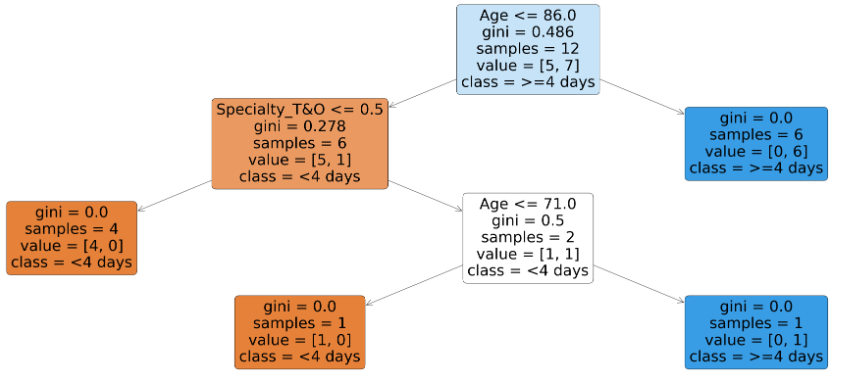
\includegraphics[scale = 0.8]{Chapters/Chapter3New/Figures/classificationtreeexample.png}
    \caption{Classification Tree for Worked Example}
    \label{fig:classificationtreeExample}
\end{figure}

% For the classification tree, a test set was generated of 20\% of the original data, equating to 3 patients. Additionally, the LOS was grouped into `$<$4 days' and `$\geq$ 4 days'.


\subsection{Extension of Random Forests}\label{sec:randomforest}
Random forests can be derived from CART models. Random forests are a bagging method which constructs decision trees on several samples, using the majority vote for classification and the mean results for regression models. The more trees there are in the forest, the more accurate the model is likely to be and the likelihood of overfitting is reduced. The algorithm's operation is shown in Figure \ref{fig:Random Forest}.

\begin{figure}[h!]
    \centering
\begin{tikzpicture}[scale =0.75, transform shape, node distance = 4.2cm]
\node(start1)[startstop]{\parbox{3cm}{\centering Training Data 2}};
\node(start2)[startstop, left of = start1]{\parbox{3cm}{\centering Training Data 1}};
\node(start3)[startstop, right of = start1]{\parbox{3cm}{\centering Training Data n}};
\node(pro1)[process, below of = start2]{\parbox{3cm}{\centering Decision Tree 1}};
\node(pro2)[process, below of = start1]{\parbox{3cm}{\centering Decision Tree 2}};
\node(pro3)[process, below of = start3]{\parbox{3cm}{\centering Decision Tree n}};
\node(pro4)[term, below of = pro2]{\parbox{4.5cm}{\centering Voting/averaging using training data}};
\node(pro5)[term1, below of = pro4]{\parbox{3cm}{\centering Prediction}};
\draw[arrow](start2) -- (pro1);
\draw[arrow](start1) -- (pro2);
\draw[arrow](start3) -- (pro3);
\path (start1) -- node[auto=false]{\ldots}(start3);
\path (pro2) -- node[auto=false]{\ldots}(pro3);
\draw[arrow](pro1) -- (pro4);
\draw[arrow](pro2) -- (pro4);
\draw[arrow](pro3) -- (pro4);
\draw[arrow](pro4) -- (pro5);
\end{tikzpicture}
    \caption{Random Forest Example}
    \label{fig:Random Forest}
\end{figure}

The individual trees are constructed using bootstrap samples as opposed to the original sample (Algorithm \ref{Alg:Random Forest}). When it comes to classification and regression trees, the splits of the tree depends on the MSE or Gini Index, respectively. Similarly, random forests employ the Scikit-Learn library \cite{Pedregosa2011} and uses the classes `RandomForestRegressor' and `RandomForestClassifier' for regression and classification trees, respectively. 

\begin{algorithm}[h!]
\caption{Random Forests - Adapted from \cite{Schonlau2020}}\label{Alg:Random Forest}
Determine stopping criterion:\\
B = Number of subtrees\\
\While{{MSE or Gini-Index$^{n} >$}0  \normalfont{\textbf{or}}\textit{ stopping criterion not met}}{
\For{i = 1 to B}{
Draw a bootstrap sample of size N from the training data\\
\While{node size != minimum node size}{
randomly select a subset of m predictor variables from total p\\
\For{j = 1 to m}{
\If{jth predictor optimises splitting criterion}{split internal node into two child nodes\\ \textbf{break;}}
}
}
}
}
\Return the ensemble tree of all B subtrees generated in the outer for loop;
% \For{$i\gets 1$ \KwTo B}{
% {Draw a bootstrap sample of size $N$ from training data}\;
% \While{node size != minimum node size}{{
% randomly select a subset of $m$ predictor variables from total $p$}\;
% \For{$j\gets 1$ \KwTo m}{
% \If{jth predictor optimises splitting criterion}
% {split internal node into two child nodes\;
% \textbf{break;}} 
% }
% }
% }
% \Return the ensemble tree of all B subtrees generated in the outer for loop;
\end{algorithm}

\paragraph{Worked Example}\\
The working example may be used with both the random forest's regression and classification versions. Random forests often perform better when there is more data available because of their nature, allowing them to sample more decision trees. However, random forests become difficult to visualise. The number of decision trees will be displayed in accordance with the number of decision tree iterations selected. This can become too computationally expensive, though, with large numbers of iterations.

\subsection{Feature Parameters}
There are parameters and attributes within each of the four cases; $`DecisionTreeRegressor'$, $`DecisionTreeClassifier'$, $`RandomForestRegressor'$ and $`RandomForestClassifer'$, that can be changed to increase the accuracy of the predictions.
Tables \ref{tab:Paramters1} and \ref{tab:Paramters2} display the parameters and attributes options for each of the methods, with the default entry for each shown in \textcolor{blue}{blue}.
The best parameter or value to select in order to obtain the highest accuracy score can be determined by subjecting these parameters to parameter optimisation.

All four methods, share eleven of the same parameters used within the model. The criterion is a function that assesses the split's quality and ultimately determines where the split occurs. The splitter is the process used to decide whether the best split will be employed at each node, or if a random split will be selected. The maximum depth of the tree is determined by its max\_depth; if no parameter is chosen, the node expands until all of its leaves are pure or until all of its leaves include fewer than the min\_samples\_split. The min\_samples\_split are the minimum number of samples required to split an internal node. Similarly, the min\_samples\_leaf are the minimum number of samples required to be at a leaf node. Only split points that will leave two nodes with at least min\_samples\_leaf training samples will be taken into consideration. The min\_weight\_fraction\_leaf is the fraction of the input samples required to be at a leaf node. The max\_features determines the number of features to consider when looking for the best split. If \textit{auto, sqrt, log2} or \textit{None} are selected, then max\_features will be equal to the attribute \textit{n\_features}. The parameter random\_state controls the randomness of the estimator and the features are always randomly permuted at each split, even if `splitter' is set to `best'. To obtain deterministic behaviour during fitting, random\_state has to be fixed to an integer. Max\_leaf\_nodes set the maximum number of end nodes that will be constructed in the model, if no value is selected then there will be an unlimited number of leaf nodes. Min\_impurity\_decrease causes a node to be split if the split induces a decrease of the impurity greater than or equal to its value. The following equation calculates the min\_impurity\_decrease:
\begin{equation}
    \frac{N_t}{N} * (impurity - \frac{N_{t_R}}{N_t} * right\_impurity -\frac{N_{t_L}}{N_t} * left\_impurity)
\end{equation}
where $N$ is the total number of samples, $N_t$ is the number of samples at the current node, $N_{t_L}$ is the number of samples in the left child node and $N_{t_R}$ are the number of samples in the right child node. In essence, the formula accounts for the parent nodes contribution to the whole tree $\frac{N_t}{N}$. The ccp\_alpha complexity parameter, which selects the subtree with the largest cost complexity that is smaller than the ccp\_alpha value, is the final parameter that is shared by all four models.

Additionally, the `$DecisionTreeClassifer$' and `$RandomForestClassifer$ require the parameter class\_weight. This parameter can be used to account for unbalanced classes and gives a class with a high population greater weight.

The random forest algorithms require further parameters. Firstly, n\_estimators tells the user the number of trees within the model. Bootstrap determines whether samples of the data are used within the model or if the whole dataset is used. Following on, if bootstrap = True, then there is the option for oob\_score which uses out-of-bag samples to evaluate its performance. The n\_jobs parameter controls how many jobs will run concurrently, and how many processors will be available. Warm\_start allows parts of the model that were learned from previous parameter values to be reused, which ultimately saves time. Finally, max\_samples requires the user to select the number of samples to draw from X to train each base estimator, only if bootstrap = True.

\newpage
\begin{landscape}
\begin{table}[hbt!]
    \centering\scalebox{0.9}{
    \begin{tabular}{lcc} \toprule
        \textbf{Parameter} & \textbf{DecisionTreeRegressor} & \textbf{DecisionTreeClassifier}  \\\midrule
        
         criterion& ``\textcolor{blue}{squared\_error}'', ``friedman\_mse'', ``absolute\_error'', ``poisson''& ``\textcolor{blue}{gini}'',``entropy'',``log\_less''\\
         splitter & ``\textcolor{blue}{best}'', ``random''  & ``\textcolor{blue}{best}'',``random'' \\
         max\_depth & integer, (\textcolor{blue}{None})& integer, (\textcolor{blue}{None})\\
         min\_samples\_split & integer, float, (\textcolor{blue}{2}) & integer, float, (\textcolor{blue}{2})  \\
         min\_samples\_leaf & integer, float, (\textcolor{blue}{1}) & integer, float, (\textcolor{blue}{1})  \\
         min\_weight\_fraction\_leaf & Float (\textcolor{blue}{0}) & Float (\textcolor{blue}{0}) \\
         max\_features & integer, float, ``auto'', ``sqrt'', ``log2'', (\textcolor{blue}{None}) & integer, float, ``auto'', ``sqrt'', ``log2'', (\textcolor{blue}{None})\\
         random\_state & integer, ``random\_state'', (\textcolor{blue}{None}) & integer, ``random\_state'', (\textcolor{blue}{None})  \\
         max\_leaf\_nodes & integer, (\textcolor{blue}{None})& integer, (\textcolor{blue}{None})\\
         min\_impurity\_decrease & float, (\textcolor{blue}{0})& float, (\textcolor{blue}{0}) \\
         class\_weight &  (N/A) & dict, list of dicts, ``balanced'', (\textcolor{blue}{None})\\
         ccp\_alpha & non-negative float, (\textcolor{blue}{0)}&non-negative float, (\textcolor{blue}{0)}\\ \midrule
         \textbf{Attributes} & \textbf{DecisionTreeRegressor}&\textbf{DecisionTreeClassifier} \\\midrule
         classes & (N/A) & ndarray of shape or list of ndarray \\
         feature\_importances\_ & ndarray of shape& ndarray of shape\\
         max\_features & integer & integer\\
         n\_classes\_ & (N/A) & integer, list of integers \\
         n\_features\_ & integer & integer\\
         n\_features\_in & integer& integer \\
         feature\_names\_in\_ & ndarray of shape & ndarray of shape \\
         n\_outputs\_ & integer& integer \\
         tree\_ & Tree instance & Tree instance \\\bottomrule
    \end{tabular}}
    \caption{`DecisionTreeRegressor' and `DecisionTreeClassifer' associated parameters and attributes the user can select - The default variable is highlighted in \textcolor{blue}{blue}. For variables which are an integer, float or there is no default, this is listed in brackets.}
    \label{tab:Paramters1}
\end{table}

\begin{table}[hbt!]
    \centering\scalebox{0.9}{
    \begin{tabular}{lcc} \toprule
        \textbf{Parameter} & \textbf{RandomForestRegressor} & \textbf{RandomForestClassifier}  \\\midrule
        n\_estimators & integer, (\textcolor{blue}{100}) & integer, (\textcolor{blue}{100})\\
         criterion& ``\textcolor{blue}{squared\_error}'', ``absolute\_error'', ``poisson''& ``\textcolor{blue}{gini}'',``entropy'',``log\_less''\\
         max\_depth & integer, (\textcolor{blue}{None})& integer, (\textcolor{blue}{None})\\
         min\_samples\_split & integer, float, (\textcolor{blue}{2}) & integer, float, (\textcolor{blue}{2})  \\
         min\_samples\_leaf & integer, float, (\textcolor{blue}{1}) & integer, float, (\textcolor{blue}{1})  \\
         min\_weight\_fraction\_leaf & Float (\textcolor{blue}{0}) & Float (\textcolor{blue}{0}) \\
         max\_features & integer, float, ``sqrt'', ``log2'', (\textcolor{blue}{None}) & integer, float, ``sqrt'', ``log2'', (\textcolor{blue}{None})\\
         random\_state & integer, ``RandomState instance'', (\textcolor{blue}{None})  & integer, ``RandomState instance'', (\textcolor{blue}{None})  \\
         max\_leaf\_nodes & integer, (\textcolor{blue}{None})& integer, (\textcolor{blue}{None})\\
         min\_impurity\_decrease & float, (\textcolor{blue}{0})& float, (\textcolor{blue}{0}) \\
         bootstrap & bool, (\textcolor{blue}{True}) &bool, (\textcolor{blue}{True}) \\
         oob\_score & bool, (\textcolor{blue}{False}) & bool, (\textcolor{blue}{False})\\
         n\_jobs & integer, (\textcolor{blue}{None}) & integer, (\textcolor{blue}{None})\\
         warm\_start & bool, (\textcolor{blue}{False}) & bool, (\textcolor{blue}{False})\\
         ccp\_alpha & non-negative float, (\textcolor{blue}{0)}&non-negative float, (\textcolor{blue}{0)}\\ 
         max\_samples & integer, float, (\textcolor{blue}{None}) & integer, float, (\textcolor{blue}{None})\\
         class\_weight &  (N/A) & dict, list of dicts, ``balanced'',``balanced\_subsample'', (\textcolor{blue}{None})\\\midrule
         \textbf{Attributes} & \textbf{RandomForestRegressor}&\textbf{RandomForestClassifier} \\\midrule
         base\_estimator\_ & DecisionTreeRegressor & DecisionTreeClassifier\\
         estimators\_ & list of DecisionTreeRegressor & DecisionTreeClassifier\\
         classes & (N/A) & ndarray of shape, list of such arrays \\
         feature\_importances\_ & ndarray of shape& ndarray of shape\\
         n\_features\_ & integer & integer\\
         n\_features\_in & integer& integer \\
         feature\_names\_in\_ & ndarray of shape & ndarray of shape \\
         n\_outputs\_ & integer& integer \\
         oob\_score & float & float\\
         oob\_prediction\_ & ndarray of shape & ndarray of shape\\ \bottomrule
    \end{tabular}}
    \caption{`RandomForestRegressor' and `RandomForestClassifier' associated parameters and attributes the user can select - The default variable is highlighted in \textcolor{blue}{blue}. For variables which are an integer, float or there is no default, this is listed in brackets.}
    \label{tab:Paramters2}
\end{table}
\end{landscape}

\subsection{Evaluation Metrics}
To ascertain success and how well the model predicts LOS, a series of evaluation measures can be applied to each of the different CART models.

\subsubsection{Regression Models}\\
The same coefficient of determination ($R^2$) metric can be used to compare the regression tree and random forest regression models. 
\textcolor{blue}{}

Recall the linear regression equation, Equation \eqref{eq:r2value}. This equation can be modified to create an equation for calculating success when using regression trees (Equation \eqref{Eq:R2}) \textcolor{blue}{\cite{Chicco2021}}.

\begin{equation}\label{Eq:R2}
    R^{2} = 1 - \frac{\sum^n_{i=1} (Y_{i}- \hat{Y}_{i})}{\sum^{n}_{i=1} (Y_{i} -\bar{Y}_{i})}
\end{equation}

% \begin{align}\label{Eq:R2}
%     R^{2} &= 1 - \frac{u}{v} \\
%      u &= \sum^{n}_{i=1}2 * \big(Y_{i} - \hat{Y}_{i}\big) \\
%      v &= \sum^{n}_{i=1}2* \big(Y_{i} -mean(\hat{Y}_{i})\big)
% \end{align}
where $Y_{i}$ represents the true $y$ value, $\hat {Y}_i$ is the value of the predicted $y$ value, $\bar Y_{i}$ represents the mean of all values and $n$ is the total number of observations. The higher the $R^{2}$ value, the more reliable the model is.

To calculate the $R^{2}$ for the random forest, the average $R^{2}$ is calculated (Equation \eqref{eq:forestequation}) 
\begin{equation}\label{eq:forestequation}
    R^{2}_{average} = \frac{1}{k}\sum_{i=1}^{k}R^{2}_{k}
\end{equation}
where $k$ is the number of decision trees selected to combine to the random forest.

\paragraph{Worked Example}\\
A test set of 20\%, or three patients, was included in the regression example so that the accuracy could be assessed. Three patients were chosen at random, and their LOS's were 3, 1, and 1. The predicted values for each of these variables were 3, 1 and 1, respectively. Therefore, the $u$ term is equal zero when computing $R^{2}$ from Equation \eqref{Eq:R2} and as a result, $R^{2}$ is equal to one.

The random forest regression model generated a negative $R^{2}$ score. This would imply that the model is not a very good predictor for LOS. The negative score is caused by $\sum^n_{i=1} (Y_{i}- \hat{Y}_{i}) >\sum^{n}_{i=1} (Y_{i} -\bar{Y}_{i})$.


\subsubsection{Classification Models}\\
Some of the same metrics used for logistic regression analysis can also be used to analyse the classification tree and random forest (classification) models.

The TP, FP, TN and FN rates will be obtained from Table \ref{tab:ConfusionMatrix}, which will then be used to calculate the precision, recall and accuracy as follows \cite{Baratloo2015}:

\begin{align}
    \text{Precision} &= \frac{TP}{TP + FP}\tag{\ref{eq:precision} revisited}\\
    \text{Recall} &= \frac{TP}{TP + FN}\tag{\ref{eq:recall} revisited}\\
    \text{Accuracy} &= \frac{TN + TP}{TN + FP + TP + FN} \tag{\ref{eq:accuracy} revisited}
\end{align}

The accuracy scoring method will be the primary one employed because it takes into account both the TP and TN values to determine how accurate the prediction is. When all decision trees are performed on the testing set, the answer that appears the most frequently is chosen as the final result.

Using CART models for prediction has several benefits because they can automatically identify key variables and the order in which they should be prioritised. The algorithm also generates a visual representation of the decision tree which simplifies and clarifies the final result. The tree structure, however, might become unstable and introduce variance if the dataset experiences even a slight shift. If some classes are unbalanced, it is also possible to produce under or over fitted trees.

Due to the averaging of the outcome, using random forests might increase accuracy by eliminating under or over fitting. However, the larger size challenge necessitates more computational time and resources.
\paragraph{Worked Example}\\
A test set consisting of 20\% of the original data, or three patients, was created for the classification tree. Due to the seed within the code being set to 0 to guarantee findings are reproducible, the three selected patients were the same as those in the regression tree example.
The patients LOS was 3,1 and 1 days. All three patients were predicted to be in the `$<$4 days' category. As a result, TN, FP and FN rates are all equal to zero, while the TP rate is equal to three. Consequently, the values for precision, recall and accuracy are all equal to one.

A maximum of four leaf nodes were used in the random forest classification algorithm's analysis of the data. It is interesting to note that the TP rate and FN rates were both calculated to be two, while the TN and FP rates were both zero. The model's recall therefore stands at 0.67. This would imply that utilising the straightforward classification tree yields superior outcomes in this instance.

%\section{Clustering?}

\section{Python Development}\label{sec:python}
The development of the linear regression, logistic regression and the CART models was executed within Python (Version 3.8.9). It is advantageous to utilise Python, an open source programming software, for data analysis and data visualisation when there are large amounts of data.

Using the Pandas library \cite{McKinney2010} (Version 1.2.0), the hospital admission data may be imported into Python as a dataframe. Additionally the library, statsmodels.api \cite{Perktold2022} (Version 0.12.2), was utilised to create statistical models. There is a list of additional libraries that are needed in the corresponding code. Data can then be subjected to analysis to identify patterns within the data.

\subsection{Linear Regression}
Depending on whether the independent variables are continuous or categorical, there are two coding strategies that can be used for linear regression models.

\subsubsection{Linear Regression - Continuous Independent Variable}\\
The following gives an illustration of how the linear regression model can be built with a continuous independent variable:
\begin{lstlisting}[language = python]
import pandas as pd
import statsmodels.api as sm
x = df['Age'] #Independent variable
y = df['LOS'] #Dependent variable
x=sm.add_constant(x) #Ensures there is a constant term
model = sm.OLS(y, x).fit() #Using Ordinary Least Squares method
print(model.summary())
\end{lstlisting}

Figure \ref{fig:OLSConLinReg} presents the relevant outputted results. According to Equation \eqref{eq:linreg}, the `coef' term specifies how much an increase in one unit will increase the total dependent variable.
To confirm that the results are statistically significant, it is also crucial to look at the p value, which is shown in Figure \ref{fig:OLSConLinReg} as `P$> |$t$|$'. The $R^{2}$ and the adjusted $R^{2}$ values can also be extracted directly from this table.


\begin{figure}[h!]
    \centering
    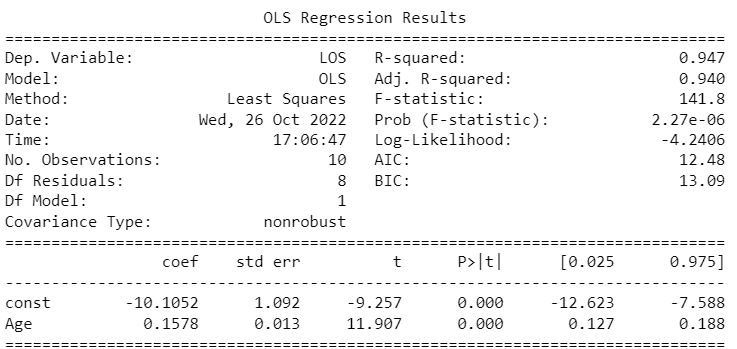
\includegraphics{Chapters/Chapter3New/Figures/OLS Results1.png}
    \caption{\textcolor{blue}{Excerpt of the OLS Results for Continuous Linear Regression}}
    \label{fig:OLSConLinReg}
\end{figure}



\subsubsection{Linear Regression - Categorical Independent Variable}\\
Similar coding methods can be applied for those variables which are categorical, with the addition of one-hot encoding.

\begin{lstlisting}[language = python]
import pandas as pd
import statsmodels.api as sm
x = df['Hospital'] #Independent variable
x = pd.get_dummies(data=x) #Applying one-hot encoding
y = df['LOS'] #Dependent variable
model = sm.OLS(y, x).fit() #Using Ordinary Least Squares method
print(model.summary())
\end{lstlisting}

Figure \ref{fig:OLSCatLinReg} contains the outputted findings. The fundamental distinction between categorical and continuous coefficients is that, if one exists, the constant term is increased by a value of either "-0.6667" or "2.3333" depending on which of the categorical coefficients is present.

\begin{figure}[h!]
    \centering
    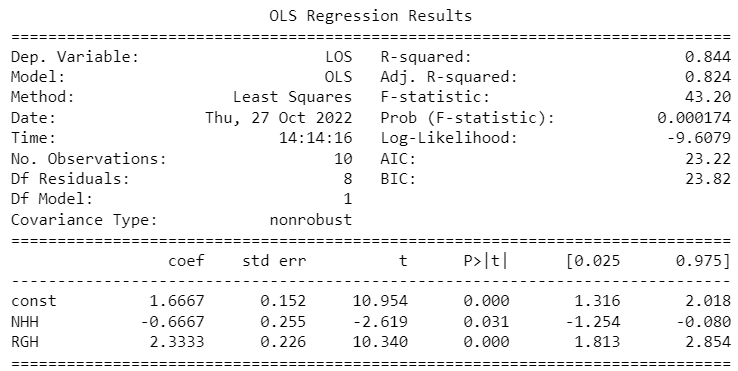
\includegraphics{Chapters/Chapter3New/Figures/OLS Results - Cat1.png}
    \caption{\textcolor{blue}{Excerpt of the OLS Results for Categorical Linear Regression}}
    \label{fig:OLSCatLinReg}
\end{figure}

\subsection{Logistic Regression}
Depending on whether the independent variables are continuous or categorical, two coding strategies for the logistic regression models can be used, adapting from the prior linear regression models.

\subsubsection{Logistic Regression - Continuous Independent Variable}
The following gives an illustration of how the logistic regression model might be used with a continuous independent variable:

\begin{lstlisting}[language = python]
import statsmodels.formula.api as smf
import numpy as np
import matplotlib.pyplot as plt
import pandas as pd
from statsmodels.formula.api import logit
from sklearn.metrics import roc_auc_score, roc_curve

conditions = [(df['LOS'] <4),(df['LOS'] >=4)] #Creating grouped LOS
values = [0,1] #Assinging values to the new groups 
df['LOS_group'] = np.select(conditions,values) #Creating LOS_group column
model = smf.logit("LOS_group ~ Age", data = df)
results = model.fit_regularized()
results.summary()

results.pred_table() #Prints confusion matrix

def plot_roc_curve(Y_test, model_probs): #Create ROC curve function
    random_probs = [0 for _ in range(len(Y_test))] 
    model_auc = roc_auc_score(Y_test, model_probs) #Calculate AUC
    random_fpr, random_tpr, _ = roc_curve(Y_test, random_probs) #Calculate ROC Curve for Random Model
    model_fpr, model_tpr, _ = roc_curve(Y_test, model_probs) #Plot ROC curves
    plt.plot(random_fpr, random_tpr, linestyle='--', label='Random')
    plt.plot(model_fpr, model_tpr, marker='.', label='Model')
    plt.plot(model_auc, label= 'AUC=%.4f' % model_auc) 
    plt.xlabel('False Positive Rate') #Plot x axis label 
    plt.ylabel('True Positive Rate') # Plot y axis label
    plt.legend()
    plt.show()
y_pred = results.fittedvalues #Determine predicted values
plot_roc_curve(df['LOS_group'], y_pred) #Plot the ROC curve
\end{lstlisting}


The associated outputted results are given in Figure \ref{fig:OLSConLogReg}. The `coef' term, which is used in linear regression as well, estimates how much an increase in one unit will result in an overall rise in the dependent variable (from Equation \eqref{eq:logreg1}). As previously stated, it is crucial to verify the p value, represented by the notation `P$> |$t$|$', to make sure the results are statistically significant. The confusion matrix and ROC curve generation instructions are also included in the code above.

\begin{figure}[h!]
    \centering
    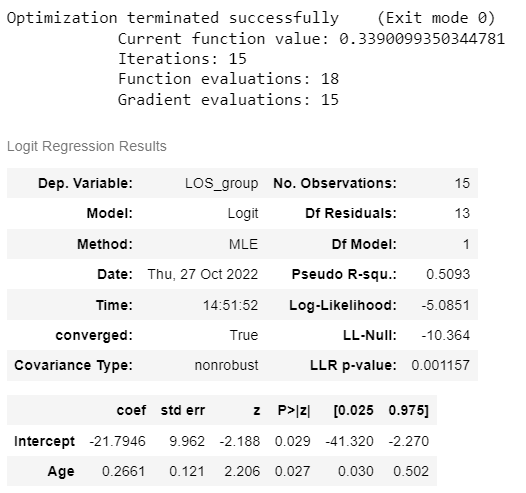
\includegraphics{Chapters/Chapter3New/Figures/Logit_cont_results.png}
    \caption{Logit Regression Results for Continuous Logistic Regression}
    \label{fig:OLSConLogReg}
\end{figure}




\subsubsection{Logistic Regression - Categorical Independent Variable}\\
The logistic regression python code for categorical variables is identical to the coding for the continuous variables, since the `logit' function can determine the type of variable inputted and act accordingly.

Furthermore, the findings of the output are very similar to those of the continuous logistic regression. The outcomes for the worked example are shown in Figure \ref{fig:OLSCatLogReg}. The number of variables contained within the independent variable, minus one, is displayed in the results. Since there was only one alternative hospital choice in this particular example, the value would simply be the intercept (i.e., -1.79 or category `0') if the hospital attended was not RGH.

\begin{figure}[h!]
    \centering
    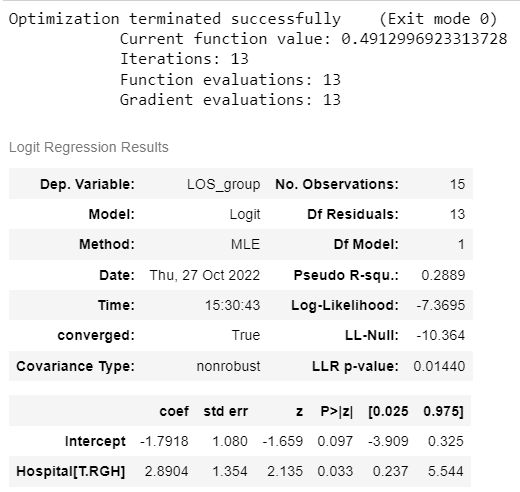
\includegraphics{Chapters/Chapter3New/Figures/Logit_cat_results.png}
    \caption{Logit Regression Results for Categorical Logistic Regression}
    \label{fig:OLSCatLogReg}
\end{figure}

\subsection{Regression Trees}\label{sec:pythonreg}
For regression trees, both the $R^{2}$ score and visualisation can be demonstrated within Python. From the original dataset entered into the notebook, the following code generates testing and training datasets. Different parameters can be entered into the 'DecisionTreeRegressor' function within this model, as detailed in Table \ref{tab:Paramters1}.
\begin{lstlisting}[language = python]
import pandas as pd
import numpy as np
import matplotlib.pyplot as plt
from sklearn.tree import DecisionTreeRegressor
from sklearn import tree
from sklearn.model_selection import train_test_split
from sklearn.tree import plot_tree
from sklearn.metrics import confusion_matrix

x = df.drop('LOS',axis = 1).copy() #Removing dependent variable from analysis
x = pd.get_dummies(x, columns = ['Hospital',
                                 'Specialty',
                                 'Admission Method',
                                 'Admission Source'
                                ]) #Applying one-hot encoding
df['LOS'] =df['LOS'].astype(float)
y = df['LOS'].copy() #Ensuring dependent variable is in own dataframe
X_train, X_test, Y_train, Y_test = train_test_split(x,y, test_size=0.2, random_state=0) #Creating training and testing data
clf_dt = DecisionTreeRegressor(random_state=0,max_leaf_nodes=4)
clf_dt.fit(X_train, Y_train) #Determines fit of the algorithm
Y_predict=clf_dt.predict(X_test)
print(clf_dt.score(X_test,Y_test)) #Prints R-squared score

plt.figure(figsize=(60,20))
plot_tree(clf_dt,
         filled=True,
         rounded=True,
         feature_names = x.columns); #Code to plot regression tree visual
plt.show()
\end{lstlisting}


\subsection{Classification Trees}\label{sec:pythonclass}
To choose the optimum splitting node, classification trees generate the Gini Index at each level using the Python class `DecisionTreeClassifier'. The following code produces testing and training datasets similarly to regression trees and uses parameters from Table \ref{tab:Paramters2} to establish the stopping criterion.

\begin{lstlisting}[language = python]
import pandas as pd
import numpy as np
import matplotlib.pyplot as plt
from sklearn import tree
from sklearn.tree import DecisionTreeClassifier
from sklearn import metrics
from sklearn.model_selection import train_test_split
from sklearn.metrics import classification_report
from sklearn.tree import plot_tree
from sklearn.metrics import confusion_matrix

conditions = [(df['LOS'] <4),(df['LOS'] >=4)] #Creating categories to predict
values = [0,1]
df['LOS_group'] = np.select(conditions,values)
x = df.drop('LOS_group', axis =1).copy() #Removing dependent variable from analysis
x =pd.get_dummies(x,columns=['Hospital',
                             'Specialty',
                             'Admission Source',
                             'Admission Method'
                             ]) #Applying one-hot encoding
df['LOS_group']=df['LOS_group'].astype(float)
y = df['LOS_group'].copy() #Ensuring dependent variable is in own dataframe

X_train, X_test, Y_train, Y_test = train_test_split(x,y, test_size=0.2, random_state=0) #Creating training and testing data

clf_dt = DecisionTreeClassifier(random_state=0,max_leaf_nodes=4) #Applying the algorithm
clf_dt.fit(X_train, Y_train) #Determines fit of algorithm
Y_predict=clf_dt.predict(X_test)
print("Accuracy:", metrics.accuracy_score(Y_test, Y_predict)) #Prints accuracy score
print(classification_report(Y_test, Y_predict)) #Prints Precision, Recall and F1 Scores
print(confusion_matrix(Y_test, Y_predict)) #Prints confusion matrix

plt.figure(figsize=(60,20))
plot_tree(clf_dt,
         filled=True,
         rounded=True,
         class_names = ['<4 days', '>=4 days'],
         feature_names = x.columns); #Code to plot classification tree visual
plt.show() 
\end{lstlisting}

\subsection{Random Forests - Regression}
The following code is adapted from the regression tree with the class changed to `RandomForestRegressor'. Due to the difficulty in visualising these trees as was previously mentioned in Section \ref{sec:randomforest}, there is no code to plot the random forest. To asses the model's fit, the $R^{2}$ is also outputted.

\begin{lstlisting}[language = python]
import pandas as pd
import numpy as np
from sklearn.metrics import accuracy_score
from sklearn.ensemble import RandomForestRegressor
from sklearn.model_selection import train_test_split
from sklearn.metrics import confusion_matrix

df['LOS'] = np.select(conditions,values)
x = df.drop('LOS', axis =1).copy() #Removing dependent variable from analysis
x =pd.get_dummies(x,columns=['Hospital',
                             'Specialty',
                             'Admission Source',
                             'Admission Method'               ])#Applying one-hot encoding

df['LOS']=df['LOS'].astype(float)
y = df['LOS'].copy() #Storing dependent variable in own dataframe

X_train, X_test, y_train, y_test = train_test_split(x, y, random_state=0,test_size=0.2, stratify=y)#Creating training and testing data

forest = RandomForestRegressor(n_estimators= 10, max_leaf_nodes =4) #Applying the algorithm
forest.fit(X_train, y_train) #Determine fit of algorithm

print(forest.score(X_test, y_test))
\end{lstlisting}


\subsection{Random Forests - Classification}
Adapting the code from the regression to the classification random forest is shown below.  To assess the random forest's fit, the score metrics are also printed.
\begin{lstlisting}[language = python]
import pandas as pd
import numpy as np
from sklearn.metrics import accuracy_score
from sklearn.ensemble import RandomForestClassifier
from sklearn.model_selection import train_test_split
from sklearn.metrics import confusion_matrix

conditions = [(df['LOS'] <4),(df['LOS'] >=4)] #Creating categories for prediction
values = [0,1]
df['LOS_group'] = np.select(conditions,values)
x = df.drop('LOS_group', axis =1).copy() #Removing dependent variable from analysis
x =pd.get_dummies(x,columns=['Hospital',
                             'Specialty',
                             'Admission Source',
                             'Admission Method'               ])#Applying one-hot encoding

df['LOS_group']=df['LOS_group'].astype(float)
y = df['LOS_group'].copy() #Storing dependent variable in own dataframe

X_train, X_test, y_train, y_test = train_test_split(x, y, random_state=0,test_size=0.2, stratify=y)#Creating training and testing data

forest = RandomForestClassifier(n_estimators= 10, max_leaf_nodes =4) #Applying the algorithm
forest.fit(X_train, y_train) #Determine fit of algorithm

y_pred_test = forest.predict(X_test)
print(forest.score(X_test, y_pred_test)) #Calculates the R squared value


\end{lstlisting}
\section{Summary}
Vast amounts of data are frequently collected by healthcare professionals but are rarely used or thoroughly evaluated. It is critical to comprehend the most recent patterns in the data in order to make informed decisions about policies and resource needs. Patients who are elderly or frail frequently differ clinically and demographically from the general adult population, and they often have more complicated medical demands. Longer hospital stays are the end outcome, along with slower recovery times and more face to face interaction with medical professionals.

This chapter has provided a comprehensive introduction of the theory underlying the most popular predictive analytical techniques presently used in healthcare. Since this chapter covered general OR approaches, a step-by-step practical example has also been included so that healthcare professionals can quickly apply these strategies to their own departments and data. To enable model adaptation and parameter optimisation, detailed executable Python code has been provided. This allows the code to be applied to any healthcare database. The theory covered in this chapter will be applied to a case study of elderly and frail patient admissions within ABUHB, in Chapter \ref{chp:Experimental Analysis}.

In the following chapter, Chapter \ref{chp:presciptive}, the use of prescriptive analytics within healthcare are discussed, namely deterministic and two-stage stochastic modelling.
\end{document}
